\documentclass{article}

\usepackage{graphicx}
\usepackage{tikz}
\usepackage{tikzsymbols}
\usetikzlibrary{calc,patterns,shapes.geometric}
\pagestyle{empty}
\usepackage[margin=0pt]{geometry}
\geometry{papersize={14in,12in}}

\def\centerarc[#1](#2)(#3:#4:#5){\draw[#1] ($(#2)+({#5*cos(#3)},{#5*sin(#3)})$) arc (#3:#4:#5);}

\begin{document}
	\begin{figure}
		\centering
		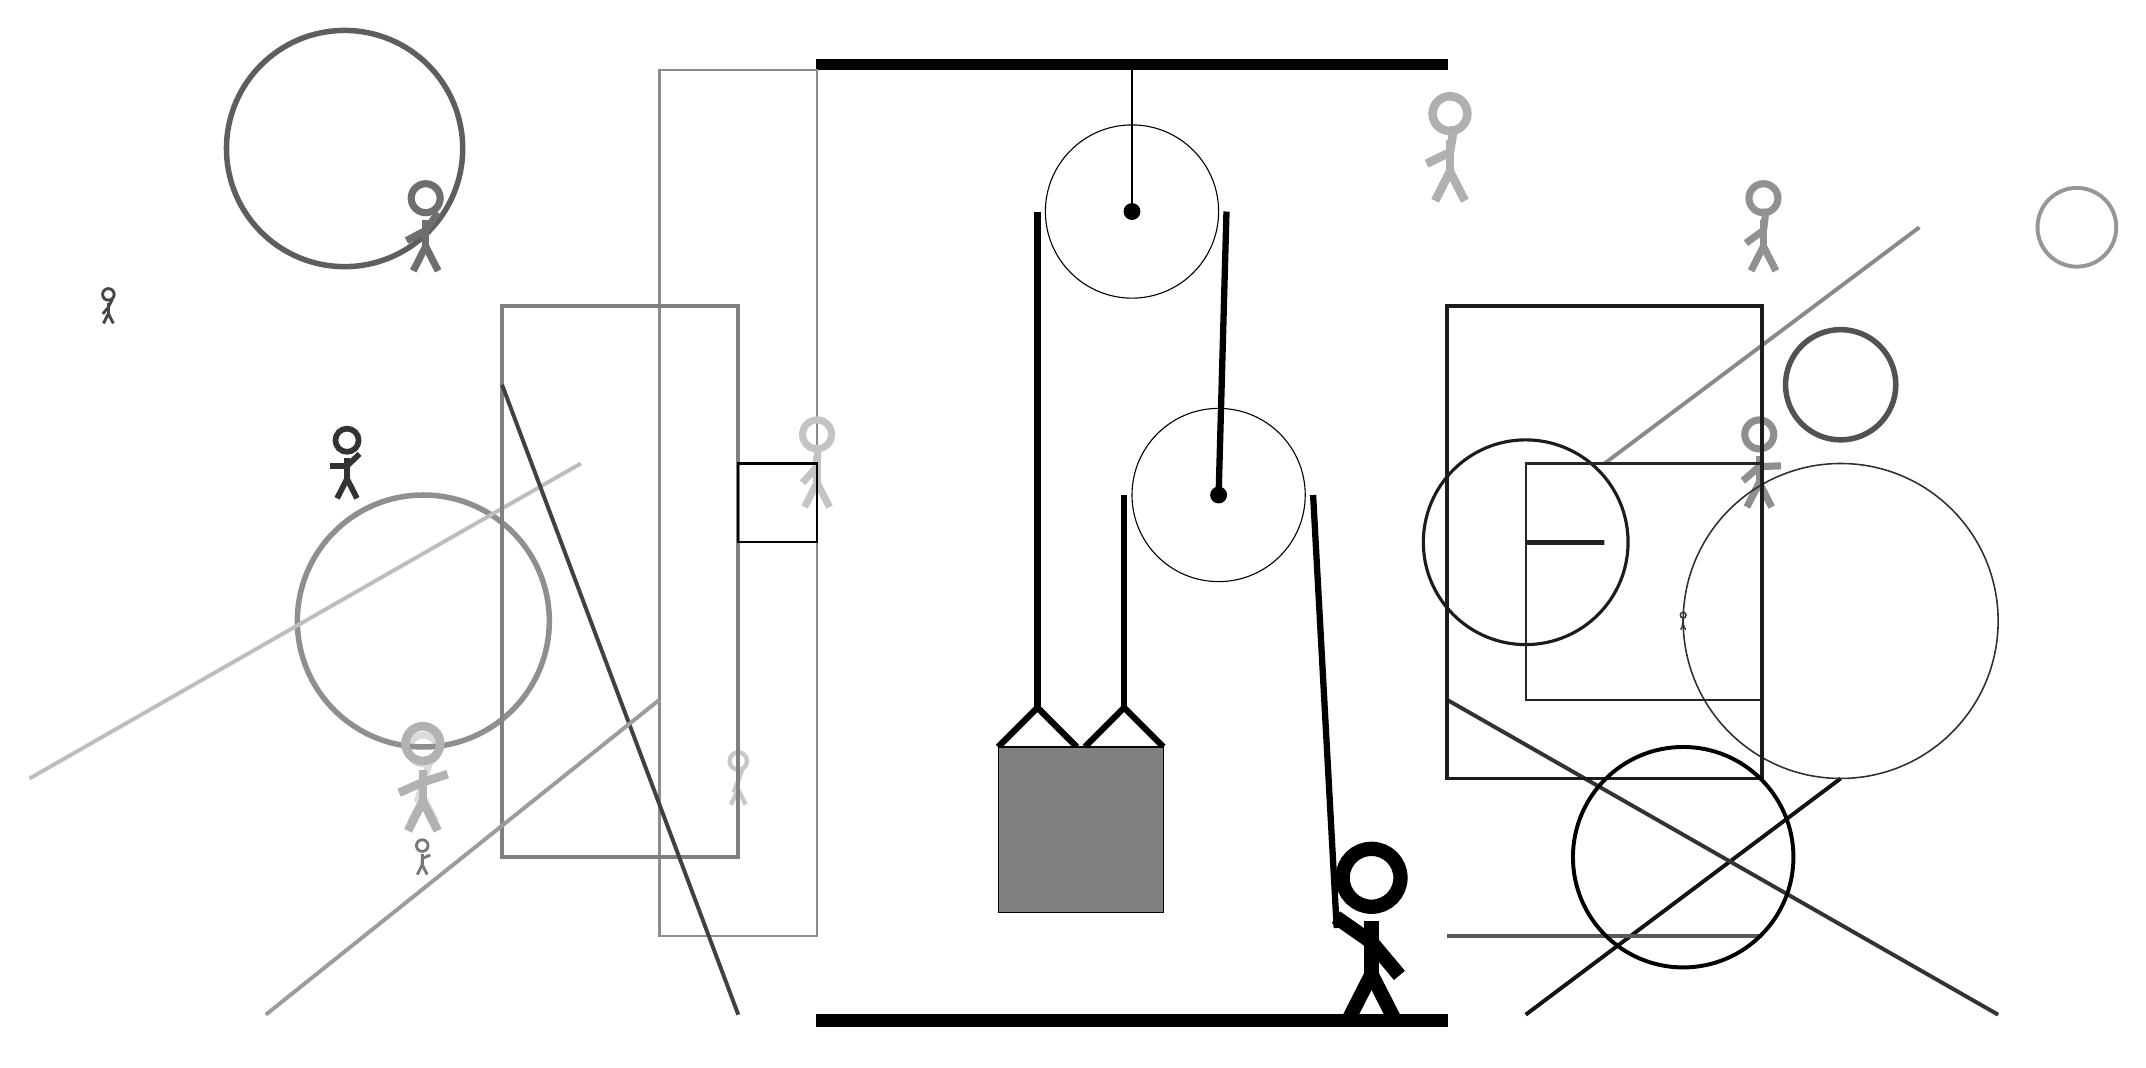
\begin{tikzpicture}
			%%%%% START %%%%%
			
			\draw[fill=black] (-2, 9) rectangle (6, 9.125);
			
			\draw (2, 7.2) circle (1.1);
			\draw[fill=black] (2, 7.2) circle (0.1);
			\draw[thick] (2, 7.2) -- (2, 9);
			
			\draw[line width=0.5mm, color=black!46](8, 4) -- (12, 7);
			
			\draw[line width=0.3mm, color=black!45] (-2, -2) rectangle (-4, 9);
			\node[line width=0.2mm, color=black!14] at (-7, 0) {\Strichmaxerl[5][74][72]};
			\draw[line width=0.5mm, color=black!47](7, 4) -- (9, 4);
			
			\draw[line width=0.5mm, color=black!93](7, -3) -- (11, 0);
			\node[line width=0.5mm, color=black!44] at (10, 4) {\Strichmaxerl[5][41][2]};
			\node[line width=0.6mm, color=black!31] at (6, 8) {\Strichmaxerl[6][26][81]};
			\draw [line width=0.7mm, color=black!63](-8, 8) circle (1.5);
			\node[line width=0.6mm, color=black!23] at (-2, 4) {\Strichmaxerl[5][48][87]};
			\draw [line width=0.5mm, color=black!41](14, 7) circle (0.5);
			\node[line width=0.4mm, color=black!80] at (-8, 4) {\Strichmaxerl[4][0][44]};
			
			\node[line width=0.6mm, color=black!22] at (-3, 0) {\Strichmaxerl[3][69][70]};
			\draw [line width=0.7mm, color=black!44](-7, 2) circle (1.6);
			\draw[line width=0.5mm, color=black!26](-5, 4) -- (-12, 0);
			\node[line width=0.6mm, color=black!30] at (-7, 0) {\Strichmaxerl[6][24][18]};
			\draw [line width=0.7mm, color=black!68](11, 5) circle (0.7);
			
			\draw[line width=0.6mm, color=black!87] (8, 3) rectangle (7, 3);
			\draw [line width=0.4mm, color=black!89](7, 3) circle (1.3);
			\draw [line width=0.2mm, color=black!81](11, 2) circle (2.0);
			
			\node[line width=0.3mm, color=black!73] at (-11, 6) {\Strichmaxerl[2][50][64]};
			\node[line width=0.5mm, color=black!81] at (9, 2) {\Strichmaxerl[1][79][86]};
			\draw[line width=0.5mm, color=black!65](6, -2) -- (10, -2);
			
			\draw[line width=0.5mm, color=black!50] (-3, -1) rectangle (-6, 6);
			\draw[line width=0.3mm, color=black!99] (-2, 4) rectangle (-3, 3);
			\node[line width=0.5mm, color=black!57] at (-7, 7) {\Strichmaxerl[5][28][55]};
			
			\draw[line width=0.3mm, color=black!85] (7, 1) rectangle (10, 4);
			\node[line width=0.7mm, color=black!53] at (-7, -1) {\Strichmaxerl[2][89][23]};
			\draw[line width=0.5mm, color=black!80](6, 1) -- (13, -3);
			\node[line width=0.4mm, color=black!43] at (10, 7) {\Strichmaxerl[5][36][83]};
			\draw[line width=0.4mm, color=black!89] (6, 0) rectangle (10, 6);
			\draw[line width=0.5mm, color=black!75](-6, 5) -- (-3, -3);
			\draw [line width=0.5mm, color=black!100](9, -1) circle (1.4);
			\draw[line width=0.5mm, color=black!39](-4, 1) -- (-9, -3);
			
			\draw (3.1, 3.6) circle (1.1);
			\draw[fill=black] (3.1, 3.6) circle (0.1);
			
			\draw[line width = 0.8mm]  (0.3, 0.4) -- (0.8, 0.9) -- (1.3, 0.4);
			\draw[line width = 0.8mm]  (1.4, 0.4) -- (1.9, 0.9) -- (2.4, 0.4);
			\draw[fill=black!50] (0.3, 0.4) rectangle (2.4, -1.7);
			
			\draw[line width = 0.8mm] (0.8, 7.2) -- (0.8, 0.9);
			\centerarc[line width = 0.8mm](2, 7.2)(0:180:1.2000000000000002);
			\draw[line width = 0.8mm] (3.2, 7.2) -- (3.1, 3.6);
			\draw[line width = 0.8mm] (1.9, 3.6) -- (1.9, 0.9);
			\centerarc[line width = 0.8mm](3.1, 3.6)(0:180:1.2000000000000002);
			\draw[line width = 0.8mm] (4.3, 3.6) -- (4.6, -1.9);
			
			\node at (5, -2) {\Strichmaxerl[10][-35][-50]};
			
			\draw[fill=black] (-2, -3) rectangle (6, -3.15);
			
			%%%%% END %%%%%
		\end{tikzpicture}
	\end{figure}	
\end{document}